\chapter{Design and implementation}
\label{design_implementation}

This chapter aims to tell the process of design and implementation of a Mining Framework. This system helps its users to 
recreate the steps done in the case studies analysis in previous chapter using a single UI. Its main goal is to automize the 
mining activity and gain a deeper control on the overall process.

This chapter is composed from section \ref{desing:overview} where the mining framework is introduced and from section 
\ref{desing:architecture} where the solution is described in detail starting from two images that depict the achitecture of the 
system and how messages are exchanged between software components. After that, these images are described in detail.


\section{Solution overview}
\label{desing:overview}
The developed Mining framework want to allow its users to extract information from the blockchain using process mining techniques 
even if they are not experts. In fact it emulates the steps applied in chapter \ref{case_studies} but hiding some complexities to 
the user: for example it is not more needed to know Disco, ProM and Apromore and how to use them. All the process is automated 
and can be started with few clicks. 

The solution is structured in two applications: a front-end and a back-end. The front-end is developed in Angular because of its 
simplicity, the great support over it and its good performances. The UI is designed for simplicity and is based on Google Material 
Design. The server is developed in java because of the need to integrate some ProM libraries for the mining algorithms 
implementation.


\section{Solution architecture}
\label{desing:architecture}

Figure \ref{images:desing_architecture} shows the architecture of the system in a component diagram.

\begin{figure}[!ht]
    \centering
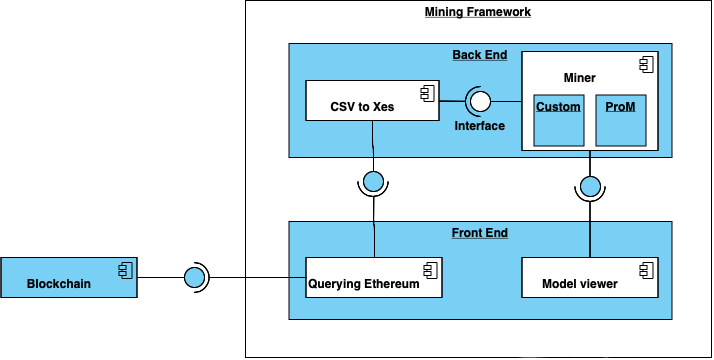
\includegraphics[width=\textwidth]{images/component_diagram.png}
    \caption{Solution architecture}
    \label{images:desing_architecture}
\end{figure}

In this diagram there are the Mining Framework and the blockchain that are two separate and independent systems which interact 
each other. Ethereum is the blockchain component for this thesis. Instead the the Mining Framework is a software solution 
composed by four main components arranged in a front-end and a back-end. These components are:

\begin{itemize}
    \item \textbf{Querying}, this component has the goal to extract data from the blockchain. It is part of the front-end 
        application so it is implemented in Angular. In order to 
        interact with the blockchain it uses Web3.js that, being a javascript library is compatible with Typescript, the 
        programming language used in Angular development. The development of this component has been inspired by the SQL 
        language: this language is used to extract integrated data from databases. In general SQL has a lot of features but only 
        a subset of them are needed in the Querying component: for example indexing, editing and creations are unusefull for the purpose of 
        the thesis. For this the "Querying component" is built as a graphical query language: it leads the user in the building of the 
        query, reducing the error probability. It has a simple and effective UI in order to make easy for users to create their queries.
        In figure \ref{images:design_query_screen} there is a screenshot taken to the application while building a query (in this
        case the query filters for all the transactions with a value grater than two and then select only few properties from the 
        filtered transactions set).

        \begin{figure}[!ht]
            \centering
        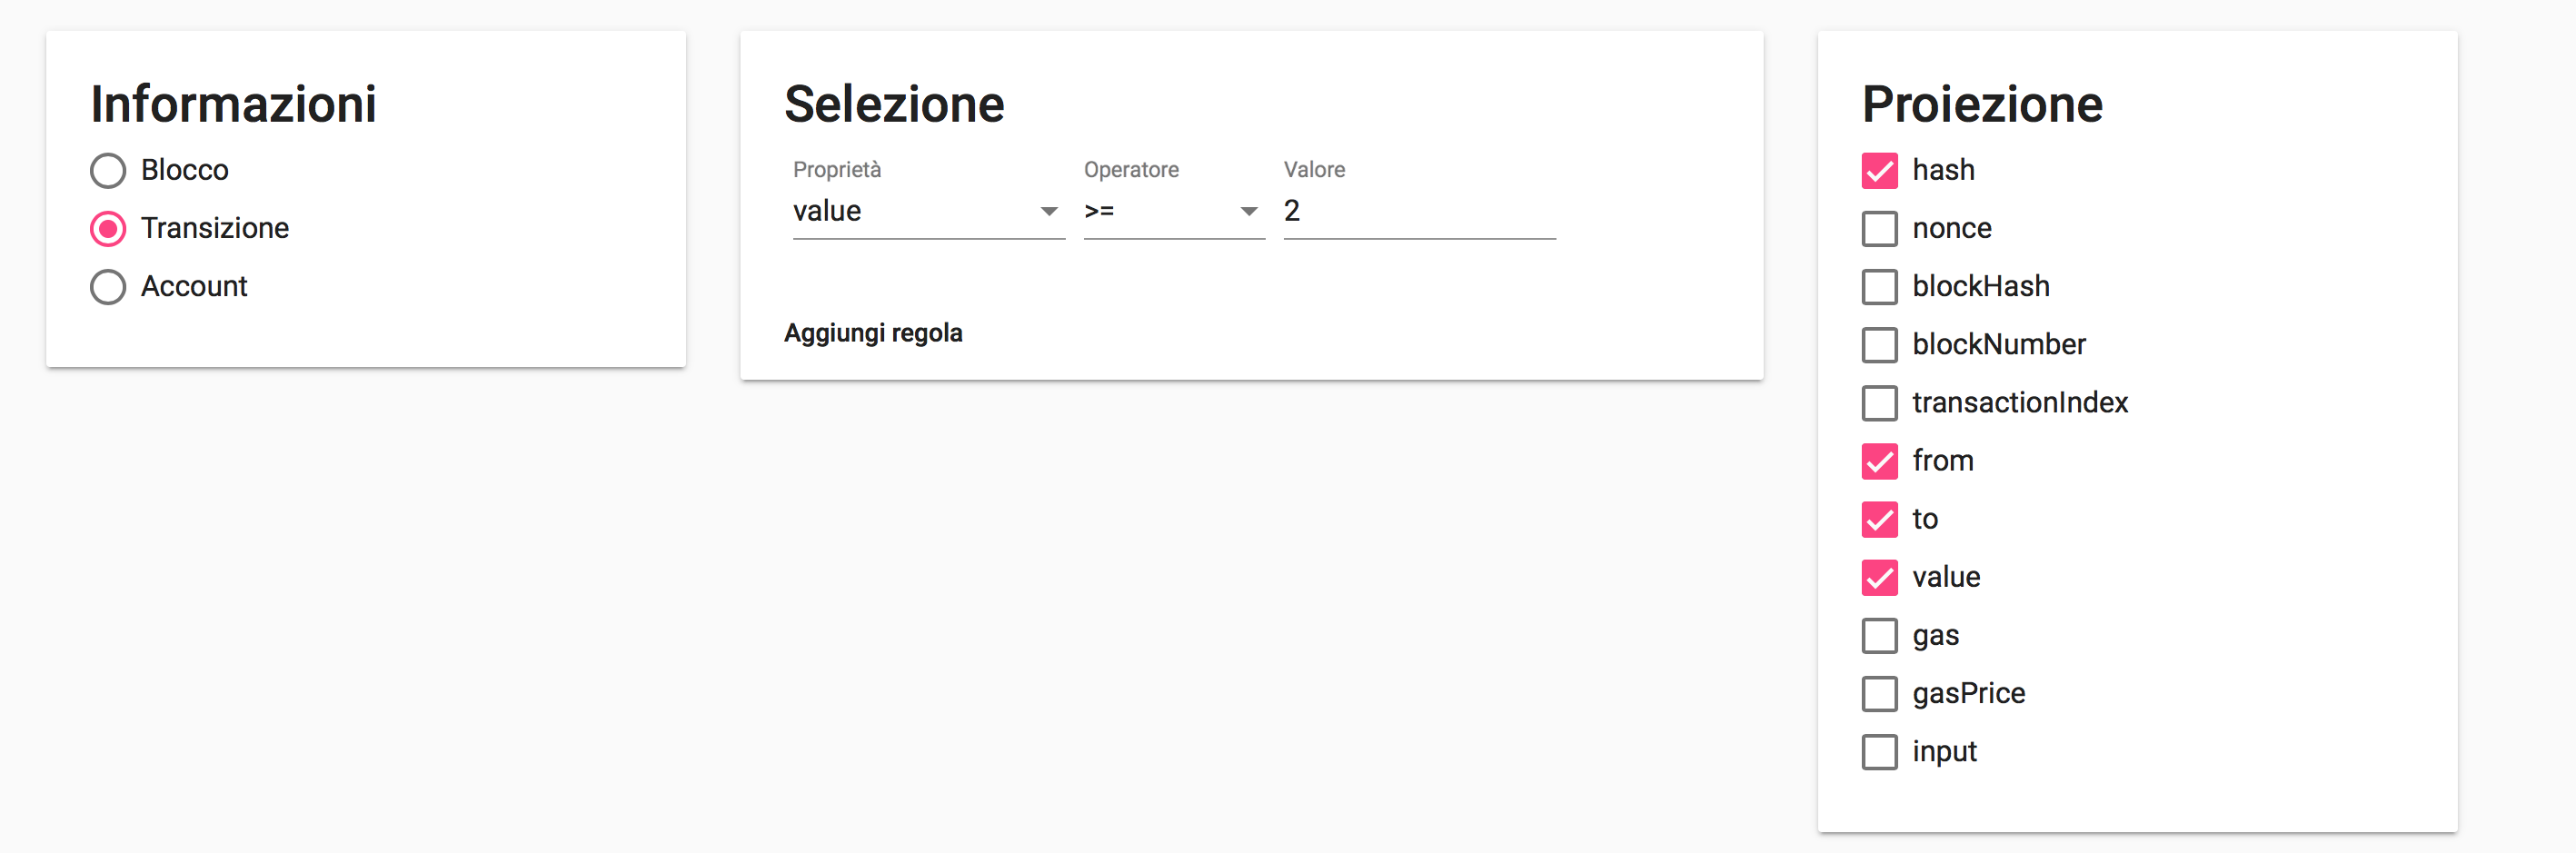
\includegraphics[width=\textwidth]{images/design_query_screen.png}
            \caption{Example of query}
            \label{images:design_query_screen}
        \end{figure}

        The application allow the user to build also complex queries using logical operators to join different simpler expressions.
        During the development some limitations, caused by the nature of the Blockchain, emerged: there are not calls that allow 
        to recover aggregated data, but only single elements are served: this means that when working with huge numbers of entities 
        the performance are really poor (every call to Web3.js api consist of a RPC call). This problem can be solved only 
        reproducing the work done by Etherscan: substantially syncing with Ethereum and creating a local db with indexes that 
        allow for fast access to all stored data. For the thesis purpose the performances are not so important so another solution 
        was adopted: partial results are shown live during the query execution. This feature does not reduce the total amount of 
        time needed to execute the query but at least gives the user a feedback about what is happening, making the application 
        usable.
        Querying allows to export query results in csv or json format.
    
    \item \textbf{CSV to Xes}, this component transform a CSV file in a Xes file. Generally it receive the results of a query 
        done with the Querying component and then produce a Xes file ready to be analyzed. This transformaion is done in the back-end 
        application beacuse here is possible to use ProM Java libraries that help in this convertion procedure.

    \item \textbf{Miner}, this component is the one responsible of the inference procedure and it is part of the back-end 
        application. It receives a Xes file and produces a model represented as Petri Net. Actually the discovery activity is based on 
        the Inductive Miner algorithm: more precisely, on the ProM implementation of the Inductive Miner. Despite this it has a 
        modular structure and more algorithms, custom or from ProM, can be easily added.

    \item \textbf{Model Viewer}, this is the component responsible for the representation of the results obtained in the mining 
        process. It receives the Petri Net infered and show it to the user.

\end{itemize}

After the presentation of the system components in Figure \ref{images:sequence_flow} is depicted a sequence diagram that 
describes the message flow between software components.

\begin{figure}[!ht]
    \centering
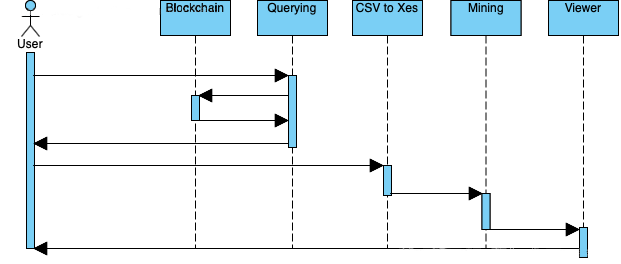
\includegraphics[width=\textwidth]{images/sequence_diagram.png}
    \caption{Message flow between system components}
    \label{images:sequence_flow}
\end{figure}

The overall process is started by the user that interacts with the Querying component: he create the query and execute it. After 
that the Querying component returns the results to the user who can choose if export these results or to use them to start a 
Mining process. In this second case data are sent to the server in CSV format: the back-end uses the converter component in order 
to obtain a Xes file that is sent to the Miner. The Miner apply the Inductive Miner algorithm and generates a Petri Net from the 
Xes file, after that it sends the Petri Net back to the client where the Model Viewer shows it.